\documentclass[hyperref={pdfpagelabel=false},usepdftitle=false,xcolor=dvipsnames]{beamer}

\usepackage[T1]{fontenc}
\usepackage[utf8]{inputenc}
\usepackage[russian]{babel}

\usepackage{amssymb, amsmath}

% table/tabular packages
\usepackage{tabularx, rotating, ragged2e, booktabs, caption}
\usepackage{graphicx}
\usepackage[verbose]{placeins}
\usepackage{blindtext}
\usepackage{multicol}

\usetheme{CambridgeUS}
\useinnertheme{rectangles}
\useoutertheme{infolines}

\newcommand\Fontvi{\fontsize{6}{7.2}\selectfont}

\beamertemplatenavigationsymbolsempty

\setbeamerfont{page number in head/foot}{size=\large}
\setbeamertemplate{footline}[frame number]
\setbeamertemplate{frametitle}[default][center]

% change font
\usefonttheme[onlymath]{serif}

\makeatother
\setbeamertemplate{headline}
{}
\makeatletter

% adding roman numerals
\makeatletter
\newcommand*{\rom}[1]{\expandafter\@slowromancap\romannumeral #1@}
\makeatother
\usepackage{makecell}
\newcolumntype{x}[1]{>{\centering\arraybackslash}p{#1}}
\usepackage{tikz}
\newcommand\diag[4]{%
  \multicolumn{1}{p{#2}|}{\hskip-\tabcolsep
  $\vcenter{\begin{tikzpicture}[baseline=0,anchor=south west,inner sep=#1]
  \path[use as bounding box] (0,0) rectangle (#2+2\tabcolsep,\baselineskip);
  \node[minimum width={#2+2\tabcolsep-\pgflinewidth},
        minimum  height=\baselineskip+\extrarowheight-\pgflinewidth] (box) {};
  \draw[line cap=round] (box.north west) -- (box.south east);
  \node[anchor=south west] at (box.south west) {#3};
  \node[anchor=north east] at (box.north east) {#4};
 \end{tikzpicture}}$\hskip-\tabcolsep}}



\usepackage{graphicx}

\begin{document}

\begin{frame}{\normalsize Поверхности потенциальной энергии межмолекулярного взаимодействия \rom{1}}
\begin{figure}
\vspace*{-0.3cm}
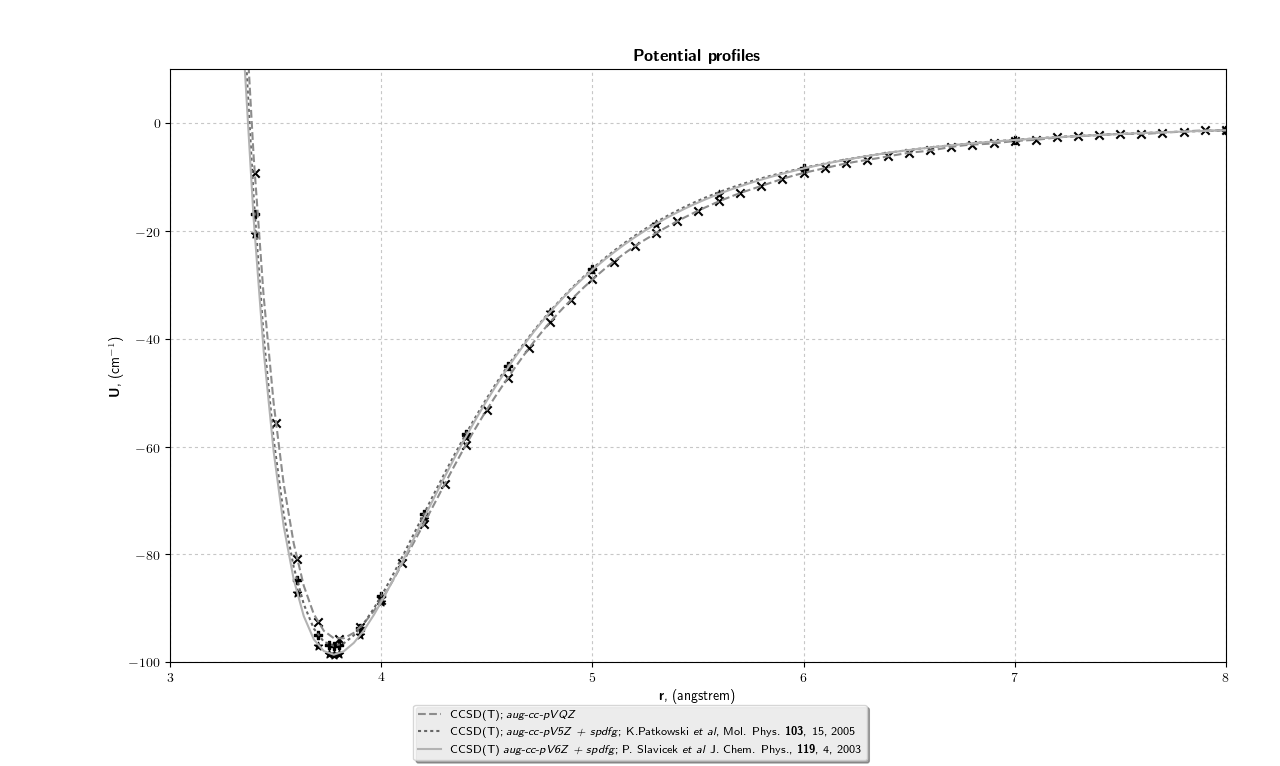
\includegraphics[width = \linewidth]{pictures/pp38.png}
\end{figure}
\end{frame}

\begin{frame}{\normalsize Поверхности потенциальной энергии межмолекулярного взаимодействия \rom{2}}
\begin{figure}
\vspace*{-0.3cm}
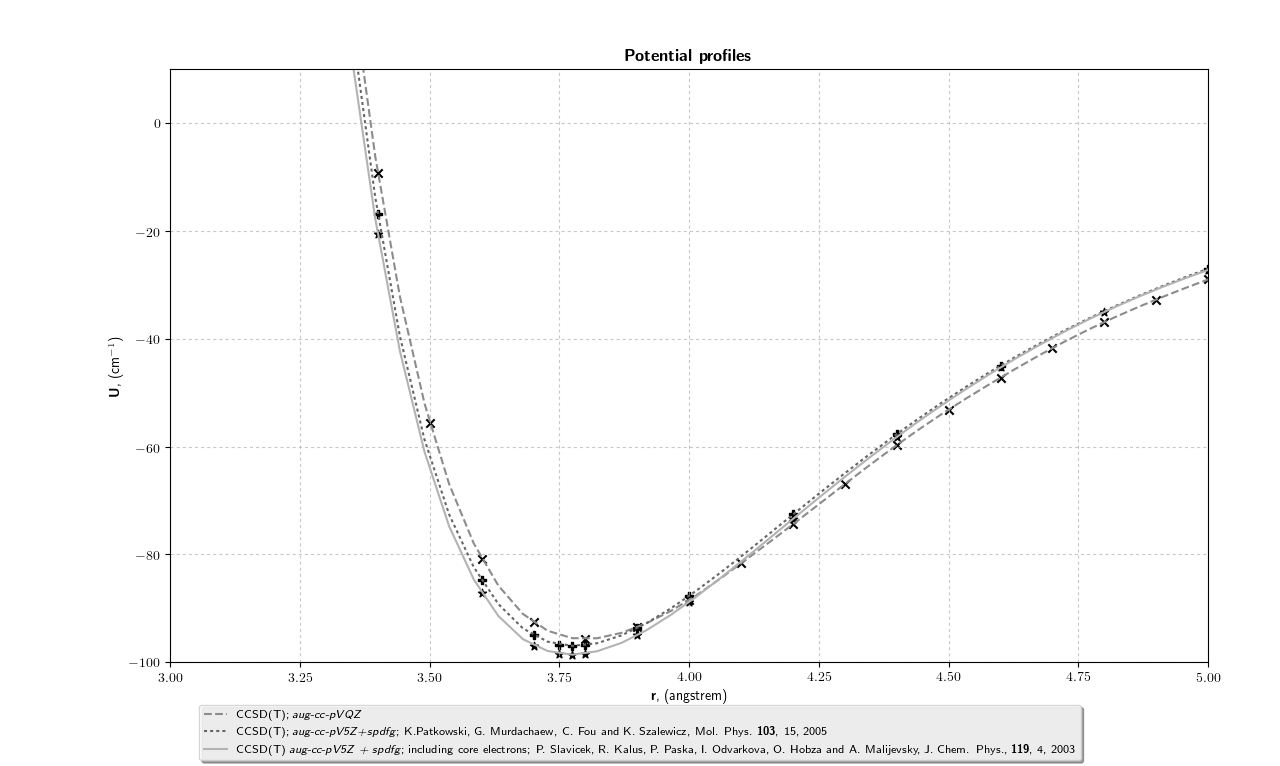
\includegraphics[width = \linewidth]{pictures/pp35.png}
\end{figure}
\end{frame}

\begin{frame}{\normalsize Поверхности потенциальной энергии межмолекулярного взаимодействия \rom{3}}
\begin{figure}
\vspace*{-0.3cm}
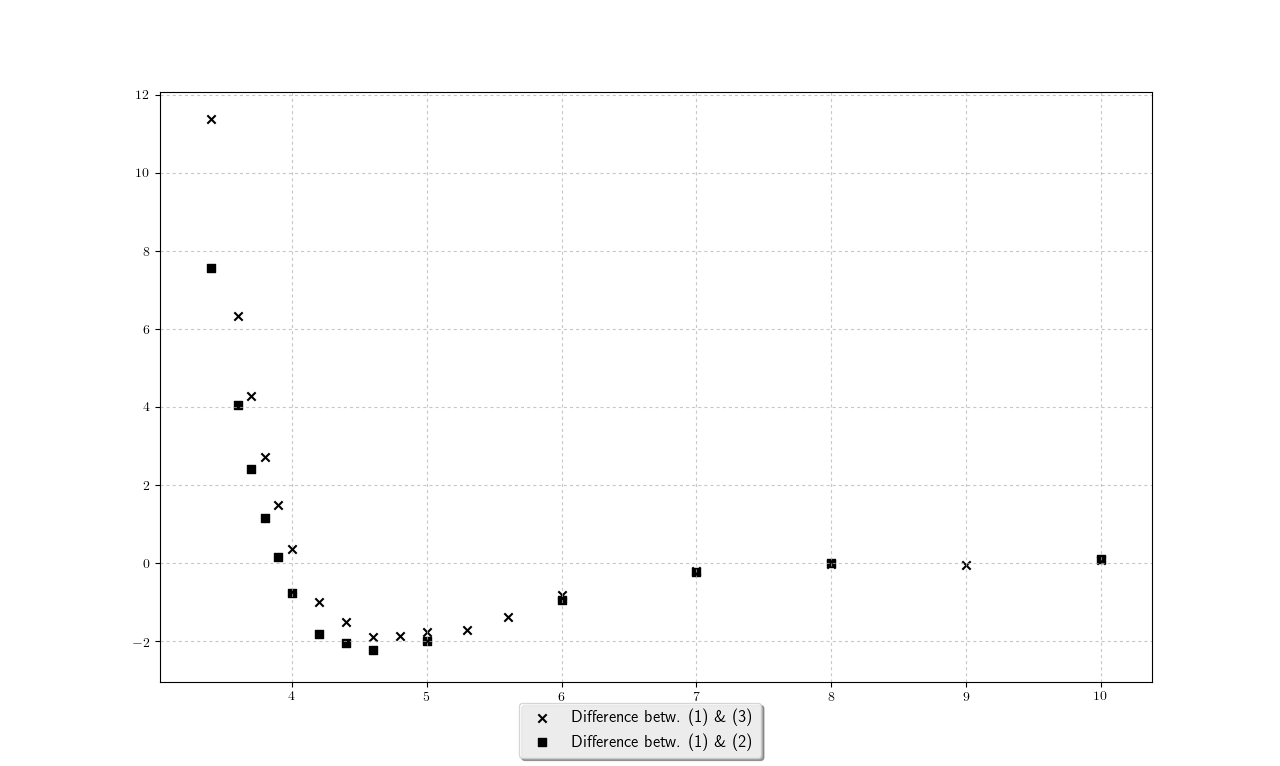
\includegraphics[width = \linewidth]{pictures/ppdiff.png}
\end{figure}
\end{frame}

\begin{frame}{\normalsize BSSE}
\begin{block}{}
\begin{gather}
\scalebox{0.8}{$EI_{AB} = E_{AB}^{opt} - E_{A}^{opt} - E_{B}^{opt} \quad \implies \quad EI_{AB} = E_{AB}^{opt} - E_{A}^{opt} - E_{B}^{opt} + \delta^{BSSE}_{AB}$} \notag \\
\scalebox{0.8}{$\delta^{BSSE}_{AB} = (E_A + E_B) - (E_A^{AB} + E_B^{AB})$} \notag
\end{gather}
\end{block}

\begin{block}{Суперпозиционная ошибка в минимуме потенциала}
\begin{center}
\begin{tabular}{cc}
\toprule
basis & $\delta^{BSSE}_{AB}$, cm$^{-1}$ \\
\midrule
\textit{aug-cc-pvdz} & 20.54 \\
\textit{aug-cc-pvtz} & 15.08 \\
\textit{aug-cc-pvqz} & 7.09 \\
\bottomrule
\end{tabular}
\end{center}
\end{block}
\end{frame}

\begin{frame}{Колебательные уровни основного состояния $Ar_2$}
\begin{center}
\begin{tabular}{cccc}
\toprule
\toprule
Transition & Exp. [1], cm$^{-1}$ & Calc., cm$^{-1}$  & Error bars, cm$^{-1}$  [1] \\
\midrule
v = 0 \rightarrow 1 & 25.69 &  24.50 & 0.02 &\\
v = 1 \rightarrow 2 & 20.58 &  19.59 & 0.02 &\\
v = 2 \rightarrow 3 & 15.58 &  14.78 & 0.02 &\\
v = 3 \rightarrow 4 & 10.91 &  10.44 & 0.03 &\\
v = 4 \rightarrow 5 & 6.84 & 6.82 & 0.07 & \\
\bottomrule
\bottomrule
\end{tabular}
\end{center}
[1]: Herman \textit{et al.} J. Chem. Phys. \textbf{89}, 4535 (1988)
\end{frame}

\begin{frame}{Вращательные уровни основного состояния $Ar_2$}
\fontsize{6pt}{7.2}\selectfont
\begin{center}
\begin{minipage}{0.4\textwidth}
\setlength{\extrarowheight}{0.1cm}
\begin{figure}
\caption*{\normalsize Emp. potential [1]}
\begin{tabular}{cccc}
\hline
\diag{.2em}{.5cm}{J}{$\nu$} & 0 & 1 & 2 \\ \hline
0 & 0.0 &  25.74 & 46.15 \\
2 & 0.35 & 26.06 & 46.44 \\ 
4 & 1.16 & 26.81 & 47.12 \\
6 & 2.43 & 27.98 & 48.18 \\
8 & 4.15 & 29.58 & 49.63 \\
10 & 6.34 & 31.59  & 51.46 \\
12 & 8.99 & 34.03 & 53.67 \\
\bottomrule
\end{tabular}
\end{figure}
\end{minipage}
\begin{minipage}{0.4\textwidth}
\setlength{\extrarowheight}{0.1cm}
\begin{figure}
\caption*{\normalsize Calc. potential}
\begin{tabular}{cccc}
\hline
\diag{.2em}{.5cm}{J}{$\nu$} & 0 & 1 & 2 \\ \hline
0 & 0.0 &  24.50 & 44.09 \\
2 & 0.34 & 24.81 & 44.37 \\ 
4 & 1.13 & 25.54 & 45.04 \\
6 & 2.37 & 26.69 & 46.10 \\
8 & 4.06 & 28.24 & 47.51 \\
10 & 6.19 & 30.22  & 49.33 \\
12 & 8.77 & 32.60 & 51.51 \\
\bottomrule
\end{tabular}
\end{figure}
\end{minipage}
\end{center}
[1]: E. A. Colbourn \textit{et al.}, J. Chem. Phys., \textbf{65}, 1741 (1976)
\end{frame}

\end{document}

